
\section{Kế hoạch thực hiện}
\label{sec:ke-hoach}

Mục này trình bày kế hoạch đưa thiết kế ở mục~3 thành một hệ thống hỗ trợ ra quyết
định hoàn chỉnh trước hạn nộp cuối kỳ (23:00 ngày 13/12/2026). Kế hoạch được xây dựng
bám theo năm tầng kiến trúc (mục~3.3) và mười chức năng hỗ trợ ra quyết định
(mục~3.5). Mỗi giai đoạn tạo ra một sản phẩm kiểm tra được và là đầu vào cho giai
đoạn kế tiếp.

% ---------------------------------------------------------------------
\subsection{Hiện trạng dự án}
\label{subsec:hien-trang}

Tính đến thời điểm báo cáo giữa kỳ, nhóm đã hoàn thành giai đoạn phân tích và thiết
kế khái niệm, cụ thể:
\begin{itemize}
    \item Xác định bối cảnh tổ chức, các vấn đề kinh doanh và người ra quyết định
          (mục~2).
    \item Khảo sát cấu trúc, đặc điểm và giới hạn của tập dữ liệu GA4 (mục~3.2).
    \item Đề xuất kiến trúc năm tầng và luồng dữ liệu của hệ thống (mục~3.3).
    \item Xây dựng bộ định nghĩa KPI thống nhất (mục~3.4) và danh sách mười chức năng
          hỗ trợ ra quyết định (mục~3.5).
    \item Ánh xạ giải pháp với vấn đề và người ra quyết định; xác định phạm vi, giả
          định và giới hạn (mục~3.6 và 3.7).
\end{itemize}

Các công việc còn lại gồm: thiết kế chi tiết mô hình chiều, xây dựng quy trình ETL,
nạp kho dữ liệu, cài đặt tầng KPI, phát triển ứng dụng hỗ trợ ra quyết định, đánh giá
hệ thống và hoàn thiện các sản phẩm nộp cuối kỳ.

% ---------------------------------------------------------------------
\subsection{Các giai đoạn thực hiện}
\label{subsec:giai-doan}

Thời gian còn lại, khoảng bảy tuần, được chia thành sáu giai đoạn nối tiếp nhau.
Giai đoạn~1 kết thúc bằng buổi thuyết trình giữa kỳ ngày 06/11/2026; slide giữa kỳ được
nộp trước một tuần, ngày 30/10/2026. Góp ý của giảng viên tại buổi thuyết trình được
dùng để điều chỉnh thiết kế ở đầu giai đoạn~2, trước khi nạp dữ liệu hàng loạt.

\subsubsection*{Giai đoạn 1: Thiết kế chi tiết và chuẩn bị giữa kỳ}
\begin{itemize}
    \item \textbf{Thời gian:} 25/10/2026 -- 06/11/2026.
    \item \textbf{Công việc chính:}
    \begin{itemize}
        \item Thiết kế chi tiết lược đồ hình sao: xác định grain, khóa và thuộc tính
              của từng bảng fact và dimension.
        \item Chốt bộ quy tắc gom nhóm source/medium thành kênh.
        \item Chốt công nghệ cho từng tầng (mục~\ref{subsec:cong-nghe}).
        \item Trích xuất thử một tuần dữ liệu để kiểm chứng thiết kế.
        \item Soạn slide giữa kỳ (nộp 30/10), tập dượt và thuyết trình (06/11).
    \end{itemize}
    \item \textbf{Sản phẩm bàn giao:} lược đồ kho dữ liệu; bảng quy tắc gom kênh;
          slide giữa kỳ.
\end{itemize}

\subsubsection*{Giai đoạn 2: Trích xuất, biến đổi và nạp dữ liệu}
\begin{itemize}
    \item \textbf{Thời gian:} 07/11/2026 -- 15/11/2026.
    \item \textbf{Công việc chính:}
    \begin{itemize}
        \item Điều chỉnh thiết kế theo góp ý giữa kỳ.
        \item Trích xuất toàn bộ 92 ngày dữ liệu về vùng lưu trữ trung gian.
        \item Làm phẳng \texttt{event\_params}, \texttt{items}; dựng phiên; chuẩn hóa
              kênh; xử lý giá trị thiếu, giá trị giữ chỗ và bản ghi trùng.
        \item Ghi nhật ký chất lượng dữ liệu.
        \item Nạp các bảng dimension, sau đó nạp các bảng fact.
    \end{itemize}
    \item \textbf{Sản phẩm bàn giao:} kho dữ liệu hoàn chỉnh; quy trình ETL; nhật ký
          chất lượng dữ liệu.
\end{itemize}

\subsubsection*{Giai đoạn 3: Xây dựng tầng KPI}
\begin{itemize}
    \item \textbf{Thời gian:} 16/11/2026 -- 22/11/2026.
    \item \textbf{Công việc chính:}
    \begin{itemize}
        \item Cài đặt các KPI ở mục~3.4 dưới dạng view/truy vấn SQL dùng chung.
        \item Kiểm thử bằng cách đối chiếu với kết quả tính trực tiếp trên dữ liệu
              nguồn.
        \item Tối ưu truy vấn: tạo chỉ mục và bảng tổng hợp theo ngày, kênh.
    \end{itemize}
    \item \textbf{Sản phẩm bàn giao:} bộ KPI đã kiểm thử; tài liệu định nghĩa KPI.
\end{itemize}

\subsubsection*{Giai đoạn 4: Phát triển ứng dụng -- bản cơ bản}
\begin{itemize}
    \item \textbf{Thời gian:} 23/11/2026 -- 29/11/2026.
    \item \textbf{Công việc chính:}
    \begin{itemize}
        \item Phát triển các chức năng 1 đến 6 ở mục~3.5 (bộ lọc đa chiều, so sánh
              hiệu suất, phân tích chất lượng kênh, phân tích phễu, drill-down).
        \item Kết nối dashboard với tầng KPI.
    \end{itemize}
    \item \textbf{Sản phẩm bàn giao:} dashboard phiên bản 1.
\end{itemize}

\subsubsection*{Giai đoạn 5: Phát triển ứng dụng -- bản hoàn chỉnh và đánh giá}
\begin{itemize}
    \item \textbf{Thời gian:} 30/11/2026 -- 06/12/2026.
    \item \textbf{Công việc chính:}
    \begin{itemize}
        \item Phát triển các chức năng 7 đến 10 (phân khúc khách hàng, cảnh báo theo
              ngưỡng, mô phỏng kịch bản, truy vết số liệu).
        \item Kiểm thử tổng thể.
        \item Đánh giá hệ thống theo các tiêu chí ở mục~3.7: tính đúng đắn của dữ liệu,
              tính nhất quán KPI, hiệu năng truy vấn, mức độ đáp ứng câu hỏi nghiệp vụ.
    \end{itemize}
    \item \textbf{Sản phẩm bàn giao:} dashboard hoàn chỉnh; kết quả đánh giá.
\end{itemize}

\subsubsection*{Giai đoạn 6: Hoàn thiện và nộp sản phẩm}
\begin{itemize}
    \item \textbf{Thời gian:} 07/12/2026 -- 13/12/2026.
    \item \textbf{Công việc chính:}
    \begin{itemize}
        \item Viết báo cáo cuối kỳ và phụ lục teamwork.
        \item Soạn slide cuối kỳ; quay và biên tập video demo 20--30 phút.
        \item Sửa lỗi phát sinh; thời gian dự phòng.
    \end{itemize}
    \item \textbf{Sản phẩm bàn giao:} báo cáo, slide (PDF) và video demo, nộp trước
          23:00 ngày 13/12/2026.
\end{itemize}

\medskip
\noindent Để theo dõi tiến độ, nhóm đặt bảy mốc kiểm soát (Bảng~\ref{tab:moc}). Mỗi mốc có tiêu
chí hoàn thành cụ thể; nhóm chỉ chuyển sang giai đoạn kế tiếp khi đạt tiêu chí, hoặc
khi đã ghi nhận phần còn tồn đọng cùng phương án xử lý.

\begin{table}[H]
    \centering
    \small
    \caption{Các mốc kiểm soát và tiêu chí hoàn thành}
    \label{tab:moc}
    \begin{tabularx}{\textwidth}{|>{\raggedright\arraybackslash}p{0.9cm}
                                 |>{\raggedright\arraybackslash}p{2.1cm}
                                 |>{\raggedright\arraybackslash}p{3.4cm}
                                 |>{\raggedright\arraybackslash}X|}
        \hline
        \textbf{Mốc} & \textbf{Ngày} & \textbf{Nội dung} & \textbf{Tiêu chí hoàn thành} \\
        \hline
        M1 & 30/10/2026 & Nộp slide giữa kỳ
           & File PDF đủ năm phần theo yêu cầu, đặt tên theo số nhóm \\
        \hline
        M2 & 06/11/2026 & Thuyết trình giữa kỳ
           & Cả ba thành viên trình bày, đúng thời lượng 10 phút; có lược đồ kho dữ
             liệu chi tiết \\
        \hline
        M3 & 15/11/2026 & Kho dữ liệu hoàn chỉnh
           & Số sự kiện, số phiên và tổng doanh thu trong kho khớp với dữ liệu nguồn,
             sau khi trừ các bản ghi đã ghi nhận trong nhật ký chất lượng \\
        \hline
        M4 & 22/11/2026 & Tầng KPI đã kiểm thử
           & Mọi KPI cho cùng kết quả khi tính từ kho dữ liệu và khi tính trực tiếp
             trên dữ liệu nguồn \\
        \hline
        M5 & 29/11/2026 & Dashboard phiên bản 1
           & Chức năng 1--6 chạy đúng; thời gian phản hồi khi thay đổi bộ lọc đạt mục
             tiêu nhóm đặt ra (dưới 3 giây) \\
        \hline
        M6 & 06/12/2026 & Dashboard hoàn chỉnh
           & Đủ mười chức năng; trả lời được các câu hỏi nghiệp vụ của người ra quyết
             định ở mục~2; có kết quả đánh giá \\
        \hline
        M7 & 13/12/2026 & Nộp sản phẩm cuối kỳ
           & Báo cáo, slide (PDF) và video demo 20--30 phút được nộp trước 23:00, đặt
             tên theo số nhóm \\
        \hline
    \end{tabularx}
\end{table}

Tiến độ tổng thể của các giai đoạn và mốc kiểm soát được minh họa bằng biểu đồ Gantt ở
Hình~\ref{fig:gantt}.

% TODO: Thay khung placeholder bên dưới bằng Gantt chart khi đã vẽ xong, ví dụ:
%   \includegraphics[width=\textwidth]{images/gantt.png}
\begin{figure}[H]
    \centering
    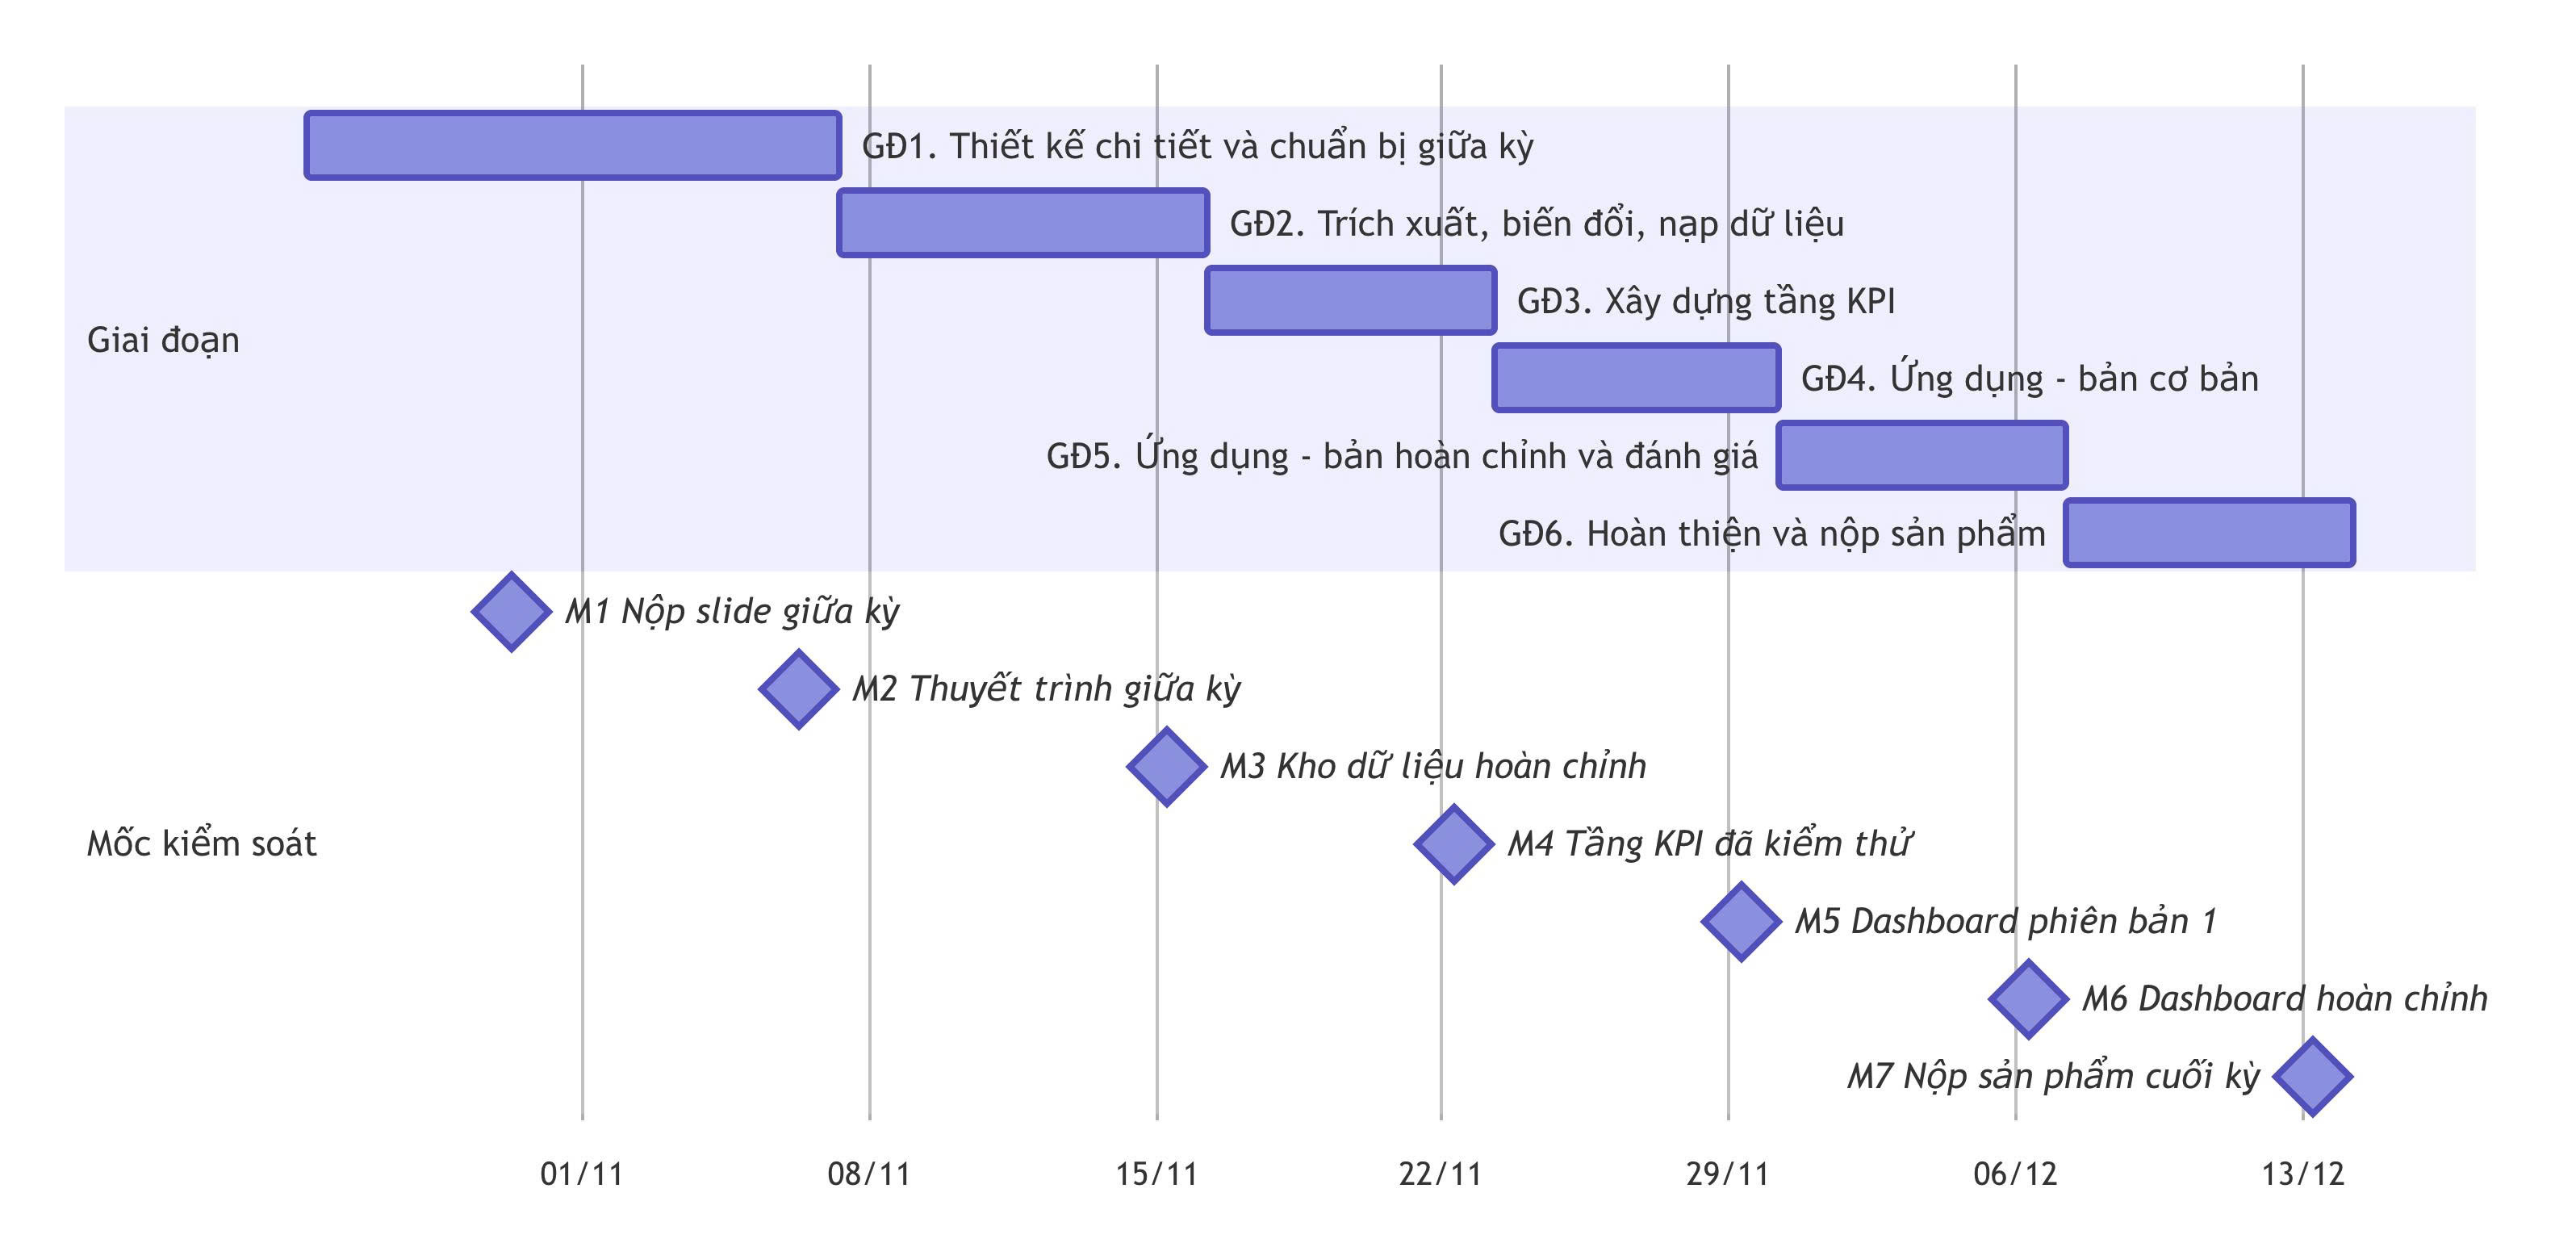
\includegraphics[width=0.9\textwidth]{image/Hien/Gantt_Chart.jpg}
    \caption{Biểu đồ Gantt kế hoạch thực hiện dự án}
    \label{fig:gantt}
\end{figure}

% ---------------------------------------------------------------------
\subsection{Phân công nhiệm vụ}
\label{subsec:phan-cong}

Nhóm phân công theo vai trò kỹ thuật, bám theo các tầng kiến trúc ở mục~3.3
(Bảng~\ref{tab:phan-cong}). Mỗi tầng có một thành viên chịu trách nhiệm chính và một
thành viên hỗ trợ, để mọi phần việc đều được rà soát chéo và có người tiếp quản khi
cần. Các sản phẩm tài liệu (báo cáo, slide, video) do cả nhóm cùng thực hiện; mỗi
thành viên trình bày phần mình phụ trách nhưng nắm được toàn bộ luồng dữ liệu, nhằm
bảo đảm đóng góp đồng đều trong các buổi thuyết trình.

% TODO: Nhóm xác nhận lại phân công vai trò bên dưới trước khi nộp.
\begin{table}[htbp]
    \centering
    \small
    \caption{Phân công vai trò và trách nhiệm}
    \label{tab:phan-cong}
    \begin{tabularx}{\textwidth}{|>{\raggedright\arraybackslash}p{2.6cm}
                                 |>{\raggedright\arraybackslash}p{2.4cm}
                                 |>{\raggedright\arraybackslash}X
                                 |>{\raggedright\arraybackslash}p{3.0cm}|}
        \hline
        \textbf{Thành viên} & \textbf{Vai trò} & \textbf{Trách nhiệm chính}
            & \textbf{Hỗ trợ} \\
        \hline
        Bùi Trọng Hiển
            & Data Engineer
            & Trích xuất dữ liệu từ BigQuery; biến đổi dữ liệu (làm phẳng, dựng phiên,
              chuẩn hóa kênh, làm sạch); nhật ký chất lượng dữ liệu; tự động hóa quy
              trình ETL
            & Nạp dữ liệu; kiểm thử mốc M3 \\
        \hline
        Nguyễn Xuân Huy Hoàng
            & Data Warehouse \& KPI Engineer
            & Thiết kế chi tiết lược đồ hình sao; nạp kho dữ liệu; cài đặt và kiểm
              thử tầng KPI; tối ưu truy vấn; chức năng truy vết số liệu
            & Bộ quy tắc gom kênh; kết nối dashboard với tầng KPI \\
        \hline
        Trần Vĩnh Dũng
            & Application Developer
            & Thiết kế giao diện và phát triển dashboard; các chức năng bộ lọc, so
              sánh, phễu, drill-down, phân khúc, cảnh báo theo ngưỡng và mô phỏng
              kịch bản
            & Kiểm thử tổng thể; biên tập video demo \\
        \hline
        Cả nhóm
            & --
            & Báo cáo, slide giữa kỳ và cuối kỳ; đánh giá hệ thống; video demo;
              thuyết trình
            & -- \\
        \hline
    \end{tabularx}
\end{table}

% ---------------------------------------------------------------------
\subsection{Công nghệ và công cụ}
\label{subsec:cong-nghe}

Công nghệ cho tầng nguồn và tầng xử lý đã được xác định. Với tầng kho dữ liệu và tầng
ứng dụng, nhóm đang cân nhắc giữa hai phương án và sẽ chốt trước ngày 30/10/2026 dựa
trên các tiêu chí ở Bảng~\ref{tab:cong-nghe}. Đánh giá sơ bộ cho thấy DuckDB phù hợp
với quy mô dữ liệu ba tháng và dễ chia sẻ giữa các thành viên, trong khi Streamlit linh
hoạt hơn cho chức năng mô phỏng kịch bản và truy vết số liệu; quyết định cuối cùng sẽ
dựa trên kết quả trích xuất thử ở giai đoạn~1.

\begin{table}[htbp]
    \centering
    \small
    \caption{Công nghệ dự kiến và tiêu chí lựa chọn}
    \label{tab:cong-nghe}
    \begin{tabularx}{\textwidth}{|>{\raggedright\arraybackslash}p{2.4cm}
                                 |>{\raggedright\arraybackslash}p{3.0cm}
                                 |>{\raggedright\arraybackslash}X
                                 |>{\raggedright\arraybackslash}p{1.8cm}|}
        \hline
        \textbf{Tầng} & \textbf{Công nghệ} & \textbf{Tiêu chí lựa chọn}
            & \textbf{Trạng thái} \\
        \hline
        Nguồn dữ liệu & Google BigQuery
            & Nơi lưu trữ sẵn tập dữ liệu GA4 & Đã chốt \\
        \hline
        Trích xuất và biến đổi & Python (pandas), SQL
            & Xử lý tốt cấu trúc lồng nhau; dễ tự động hóa và kiểm thử & Đã chốt \\
        \hline
        Kho dữ liệu & PostgreSQL hoặc DuckDB
            & Hiệu năng truy vấn phân tích; dễ triển khai và chia sẻ giữa các thành
              viên; tương thích với công cụ dashboard & Chốt trước 30/10 \\
        \hline
        Ứng dụng hỗ trợ ra quyết định & Power BI hoặc Streamlit
            & Mức độ tương tác cho người ra quyết định, đặc biệt với ngưỡng cảnh báo
              do người dùng cấu hình, mô phỏng kịch bản và truy vết số liệu; khả năng
              drill-down; thuận tiện khi demo & Chốt trước 30/10 \\
        \hline
        Cộng tác & GitHub, Overleaf, Google Drive
            & Quản lý mã nguồn và rà soát chéo; soạn báo cáo chung; lưu trữ tài liệu
            & Đã chốt \\
        \hline
    \end{tabularx}
\end{table}
\newpage
% ---------------------------------------------------------------------
\subsection{Quản lý rủi ro}
\label{subsec:rui-ro}

Bảng~\ref{tab:rui-ro} liệt kê các rủi ro chính có thể ảnh hưởng đến tiến độ và chất
lượng, cùng phương án phòng ngừa.

\begin{table}[htbp]
    \centering
    \small
    \caption{Các rủi ro chính và phương án xử lý}
    \label{tab:rui-ro}
    \begin{tabularx}{\textwidth}{|>{\raggedright\arraybackslash}p{5.2cm}
                                 |>{\raggedright\arraybackslash}p{2.1cm}
                                 |>{\raggedright\arraybackslash}X|}
        \hline
        \textbf{Rủi ro} & \textbf{Mức độ} & \textbf{Phương án xử lý} \\
        \hline
        Chất lượng dữ liệu nguồn làm sai lệch KPI
            & Cao & Kiểm chứng sớm và ghi nhật ký chất lượng dữ liệu \\
        \hline
        Trễ tiến độ giữa các giai đoạn
            & Trung bình & Theo dõi theo mốc; phát triển song song trên dữ liệu mẫu \\
        \hline
        Hiệu năng truy vấn chưa đáp ứng tính tương tác
            & Trung bình & Tối ưu truy vấn và dùng bảng tổng hợp \\
        \hline
        Phạm vi công việc vượt khả năng
            & Trung bình & Ưu tiên các chức năng cốt lõi trước \\
        \hline
        Thành viên quá tải vào cuối kỳ
            & Cao & Dành thời gian dự phòng; rà soát chéo để hỗ trợ lẫn nhau \\
        \hline
    \end{tabularx}
\end{table}

% ---------------------------------------------------------------------
\subsection{Phối hợp và theo dõi tiến độ}
\label{subsec:phoi-hop}

Để bảo đảm kế hoạch được thực hiện đúng, nhóm áp dụng các nguyên tắc sau:
\begin{itemize}
    \item \textbf{Họp định kỳ hằng tuần:} cập nhật tiến độ so với các mốc kiểm soát,
          xác định vướng mắc và điều chỉnh phân công khi có giai đoạn bị chậm.
    \item \textbf{Quản lý mã nguồn:} mỗi thành viên làm việc trên nhánh riêng trên
          GitHub; mã nguồn được thành viên hỗ trợ rà soát trước khi gộp vào nhánh
          chính.
    \item \textbf{Kiểm soát theo mốc:} mỗi mốc M1--M7 được nghiệm thu theo tiêu chí ở
          Bảng~\ref{tab:moc} trước khi chuyển giai đoạn.
    \item \textbf{Ghi nhận đóng góp:} công việc và mức độ hoàn thành của từng thành
          viên được ghi lại hằng tuần, làm cơ sở cho phụ lục báo cáo hoạt động nhóm
          (Teamwork report) trong báo cáo cuối kỳ.
\end{itemize}